\documentclass[10pt,A4paper,tikz,border=10pt]{standalone}
\usepackage[utf8]{inputenc}
\usepackage[T1]{fontenc}
\usepackage{amsmath}
%\usepackage{amsfonts}
\usepackage{amssymb}
\usepackage{mathtools}
\DeclarePairedDelimiter\abs{\lvert}{\rvert}
\usepackage{tikz}
\usetikzlibrary{shapes,arrows,shapes.misc,shapes.symbols}
\usetikzlibrary{positioning}
\usepackage{gitinfo2}
\usepackage{graphicx}

\makeatletter
\AddToShipoutPictureBG{%
	\AtPageLowerLeft{%
		\kern2.6cm
		\raisebox{\dimexpr.5\paperheight-.8\height}
		{\rotatebox{90}{\gitMarkFormat\gitMarkPref{} \textbullet{} \gitMark}}%
	}%
}%
\makeatother
\newcommand{\prdfrazioni}{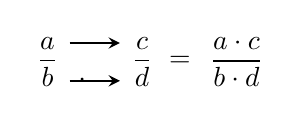
\begin{tikzpicture}[thick]
		\def\x{2.8mm}
		\def\h{2.4mm}
		\def\dist{12mm}%1cm
		\node at (0,0) {$\displaystyle \frac{a}{b}$};
		\node at (\dist,0) {$\displaystyle \frac{c}{d}$};
		\node at (1.4*\dist,0) {$\displaystyle =$};
		\node at (2.0*\dist,0) {$\displaystyle \frac{a\cdot c}{b\cdot d}$};
		% collegamento termini
		\draw[-stealth] (\x, \h)--(\dist-\x,\h); 
		\draw[-stealth] (\x,-\h)--node [near start] {$\cdot$}(\dist-\x, -\h);
	\end{tikzpicture}%
}
%\renewcommand{\gitMarkFormat}{\color{blue}\sffamily\bfseries}
\begin{document}
\tikzset{
	decision/.style={diamond, draw, %fill=blue!20,
		text width=5.5em, text badly centered, 
		%node distance=2.5cm
		, inner sep=0pt
	},
	block/.style={rectangle, draw, %fill=blue!20,
		text width=15em, 
		text centered, 
		%node distance=2.0cm,
		%rounded corners, 
		%minimum height=3em
	},
	loop/.style={chamfered rectangle,chamfered rectangle 	xsep=2cm, draw, %fill=blue!20,
		text width=15em, text centered,  
		node distance=2.5cm,% minimum height=3em
	},
	cloud/.style={draw, ellipse,%fill=red!20, 
		%node distance=1.5cm,
		 minimum height=2em
	},
	input/.style={ % requires library shapes.geometric
		draw,
		%node distance=1.5cm,
			text width=15em, text centered,  
		trapezium,
		trapezium left angle=60,
		trapezium right angle=120,
	},
	line/.style={draw, very thick, %color=black!50,
		-latex'},
	print/.style={ % requires library shapes.symbols
		draw,
		text width=14em, 
		text centered,  
		tape,
		tape bend top=none
	},
connessione/.style={
draw,
circle,
radius=5pt,
}
}
%	\begin{center}

		\begin{tikzpicture}[scale=1, %node distance = 2.5cm,
			 auto]
			% Place nodes
			\node [cloud] (init) {Inizio};
			\node [input, below of=init,node distance=2cm] (passo1) {Leggo le coordinate del punto $A(x_1,y_1)$};
	\node [input, below of=passo1, node distance=2cm] (passo2) {Leggo le coordinate del punto $B(x_2,y_2)$};		
	\node [input, below of=passo2, node distance=2cm] (passo2a) {Leggo le coordinate del punto $C(x_3,y_3)$};		
		\node [block, below of=passo2a, node distance=2cm] (passo3) {Sommo $x_1+x_2+x_3$};
		\node [block, below of=passo3, node distance=2cm] (passo4) {Sommo $y_1+y_2+y_3$};	
		\node [print, below of=passo4, node distance=2cm] (passo5) {Scrivo $B\left(\dfrac{x_1+x_2+x_3}{3},\dfrac{y_1+y_2+y_3}{3}\right)$};
		
	\node [cloud, below of=passo5, node distance=2cm] (stop) {Fine};
			\path [line] (init) -- (passo1);
			\path [line] (passo1) -- (passo2);
			\path[line](passo2)--(passo2a);
     		\path [line] (passo2a) --  (passo3);
    		\path [line] (passo3) --  (passo4);
     		\path [line] (passo4) -- (passo5);
     		\path [line] (passo5) -- (stop);
		\end{tikzpicture}
%	\end{center}
\end{document}